\documentclass[a4paper,12pt,abstracton,titlepage]{scrartcl}

\usepackage[french]{babel}
%\usepackage[T1]{fontenc}
\usepackage[utf8]{inputenc} % Umlaute, evtl. vom Betriebssystem abhaengig
\usepackage{lmodern}
\usepackage{pgfgantt}
\usepackage{titlesec}
\usepackage{float}
\usepackage{floatflt}
\usepackage{blindtext}
\usepackage{amsmath}
\usepackage{tabularx,url}
\usepackage[a4paper, left=2cm, textwidth=17cm, top=1.5cm]{geometry}
\usepackage{hyperref}


\titleformat*{\section}{\large\bfseries}
\titleformat*{\subsection}{\large\bfseries}
\titleformat*{\subsubsection}{\large\bfseries}
\titleformat*{\paragraph}{\large\bfseries}
\titleformat*{\subparagraph}{\large\bfseries}

\renewcaptionname{french}{\figurename}{Fig.}

%\titlehead{Ulm University}
%\title{Title}
%\subject{Subject}
%\author{Author}
%\publishers{%
	%\rule{\textwidth}{0.4pt} \\
	%\vspace{0.5cm}
    %\normalfont\normalsize%
    %\parbox{0.9\linewidth}{%
    %    Abstract or Introduction
    %} \\
    %\vspace{0.5cm}
   	%\rule{\textwidth}{0.4pt}
%}

\begin{document}
%\maketitle

%%% begin costom title
{\Large\noindent \emph{ESIEE Paris}}

{\Large\noindent \emph{IGI-3008}}
\begin{center}
	{\large Cryptographie	 \\ \large Léa MENERET, Fathima SAHADATTALY, Ulrike KULZER \\ \today}
\end{center}
%%% end custom title

\setcounter{page}{1} % reset page counter to one for the first page, leave the title page out

\section{Contexte}
\subsection{En général}
La cryptographie est une technique utilisée pour rendre incompréhensible à autrui un message entre un expéditeur et un destinataire. Ce procédé a notamment été utilisé en période de guerre pour permettre des attaques surprises. 
Le principe est le suivant : L'expéditeur à partir d'une clé crypte son message et l'envoie au destinataire. Celui-ci possède aussi la clé qui va lui permettre ainsi de décrypter le message.

\subsection{Histoire}
La cryptographie est utilisée depuis l'Antiquité mais certaines de ces méthodes les plus abouties datent du 20e siècle. Il existe différents principes de cryptage plus ou moins compliqués tels que\\
\\
\begin{minipage}[t]{0.5\textwidth}
    \begin{itemize}
    \item \textit{le chiffre de César :}\\
    Ce procédé a été inventé lors de l'époque romaine par Jules César pour ses communications secrètes. En décalant l'alphabet par un entier donné chaque lettre est associée à une nouvelle lettre, ainsi on peut crypter le message initiale en remplaçant chaque lettre par la nouvelle lettre attribuée.
    \paragraph{}
    \item \textit{le chiffre de Vigenère :}\\
    Il a été inventé au 16e siècle par Blaise de Vigenère et est basé sur le tableau à droite. Une clé (un mot) est répétée et mis sous le message et de cette manière on peut trouver les lettres correspondantes à partir du tableau.\\
    Exemple:
%\footnote{https://fr.wikipedia.org/wiki/Chiffre_de_Vigen\%C3\%A8re}
    \end{itemize}
    \begin{center}
    \raggedleft
 	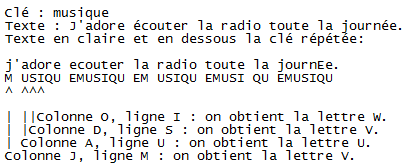
\includegraphics[height=3.4cm]{./Pictures/exempleVigenere_neuf.png}
 	%\caption{exemple du cryptage de Vigenère}
 	\label{exVig}
    \end{center} 
	
  \end{minipage} 
  \begin{minipage}[t]{0.4\linewidth}
    \raggedleft
    \strut\vspace*{-\baselineskip}\newline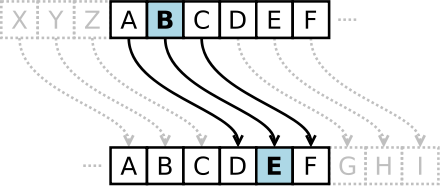
\includegraphics[width=0.9\linewidth]{./Pictures/chiffreCesar.png}
    %\caption{décalage de l'alphabet}
    \label{cesar}
    \paragraph{}
    \strut\vspace*{-\baselineskip}\newline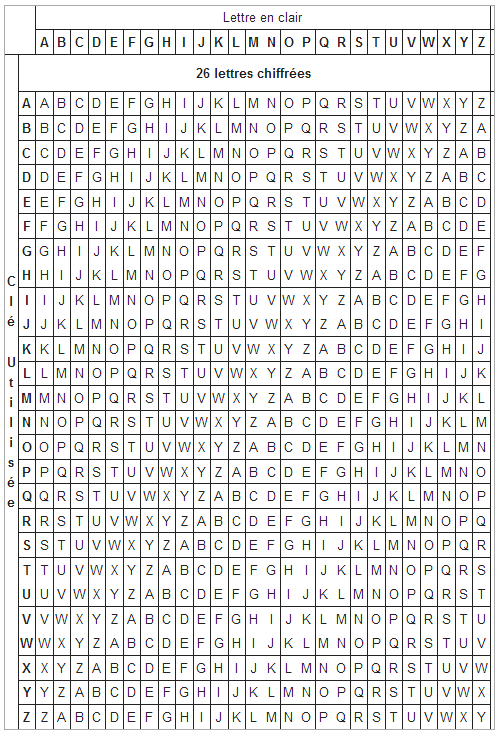
\includegraphics[width=0.9\linewidth]{./Pictures/tableauVigenere.png}
    %\caption{tableau de Vigenère}
    \label{tabVig}
  \end{minipage}

\begin{minipage}[t]{0.5\textwidth}
    \begin{itemize}
    \item \textit{celui de la machine Enigma :}\\
    L’Enigma est une machine de cryptographie inventée par Arthur Scherbius en 1919. Elle a été utilisée durant la Seconde Guerre mondiale pour la communication secrète entre les différentes unités de l’armée allemande.
La machine est constituée de cinq rotors dont un réflecteur, d’un clavier, d’un tableau de permutation et de lampes pour chaque lettre. Pour l’allumer il faut une batterie de 4,5 Volt.
Le principe est simple : Lorsqu’on appuie sur une lettre du clavier, un courant électrique va être envoyé au tableau de permutation dans lequel la lettre entrée est échangée avec une autre lettre si elles sont connectées. Puis il passera la première fois par les quatre rotors : Dans chacun des trois rotors au milieu il y a un décalage des lettres qui s’opère. À la fin les lettres sont permutées encore une fois dans le réflecteur qui les renvoie par les rotors au tableau de permutation ce qui permettra à une lampe correspondant à une lettre de s’allumer. Ainsi pour chaque lettre on relève la lettre codée, on obtient alors notre message crypté.\\
    \end{itemize}
  \end{minipage}
  \begin{minipage}[t]{0.5\linewidth}
    \raggedleft
    \strut\vspace*{-\baselineskip}\newline\newline\newline\includegraphics[width=0.9\linewidth]{./Pictures/enigma.jpg}
    %\caption{La machine Enigma}
    \label{enigma}
  \end{minipage}
  
\paragraph{}
\paragraph{}
\paragraph{}
\paragraph{}

\textit{Sites de référence :}
\begin{itemize}
\item \url{https://fr.wikipedia.org/wiki/Cryptographie}
\item \url{http://www.bibmath.net/crypto/}
\item \url{https://fr.wikipedia.org/wiki/Chiffrement_par_d\%C3\%A9calage}
\item \url{https://fr.wikipedia.org/wiki/Chiffre_de_Vigen\%C3\%A8re}
\item \url{https://fr.wikipedia.org/wiki/Enigma_(machine)}
\item photo d’Enigma:
Von William Warby from London, England - Enigma, CC BY 2.0,\\\url{https://commons.wikimedia.org/w/index.php?curid=46848023}\\
\end{itemize}



\newpage
\section{Fonctionnalité}
\subsection{Différents états du programme}
Les différents états du programme sont représentés dans le diagramme ci-dessous. Dès que le programme est lancé, il est généralement toujours dans un état en attendant des saisies de l'utilisateur. La seule exception est l'état en cryptant ou décryptant.
Sur les flèches on peut voir ce qu'il faut faire pour accéder à un autre état, soit le précédent, soit le suivant.
Avant que le programme est fermé, il affichera un petit message de remerciement.\\

\begin{figure}[tpbh]
	\centering
  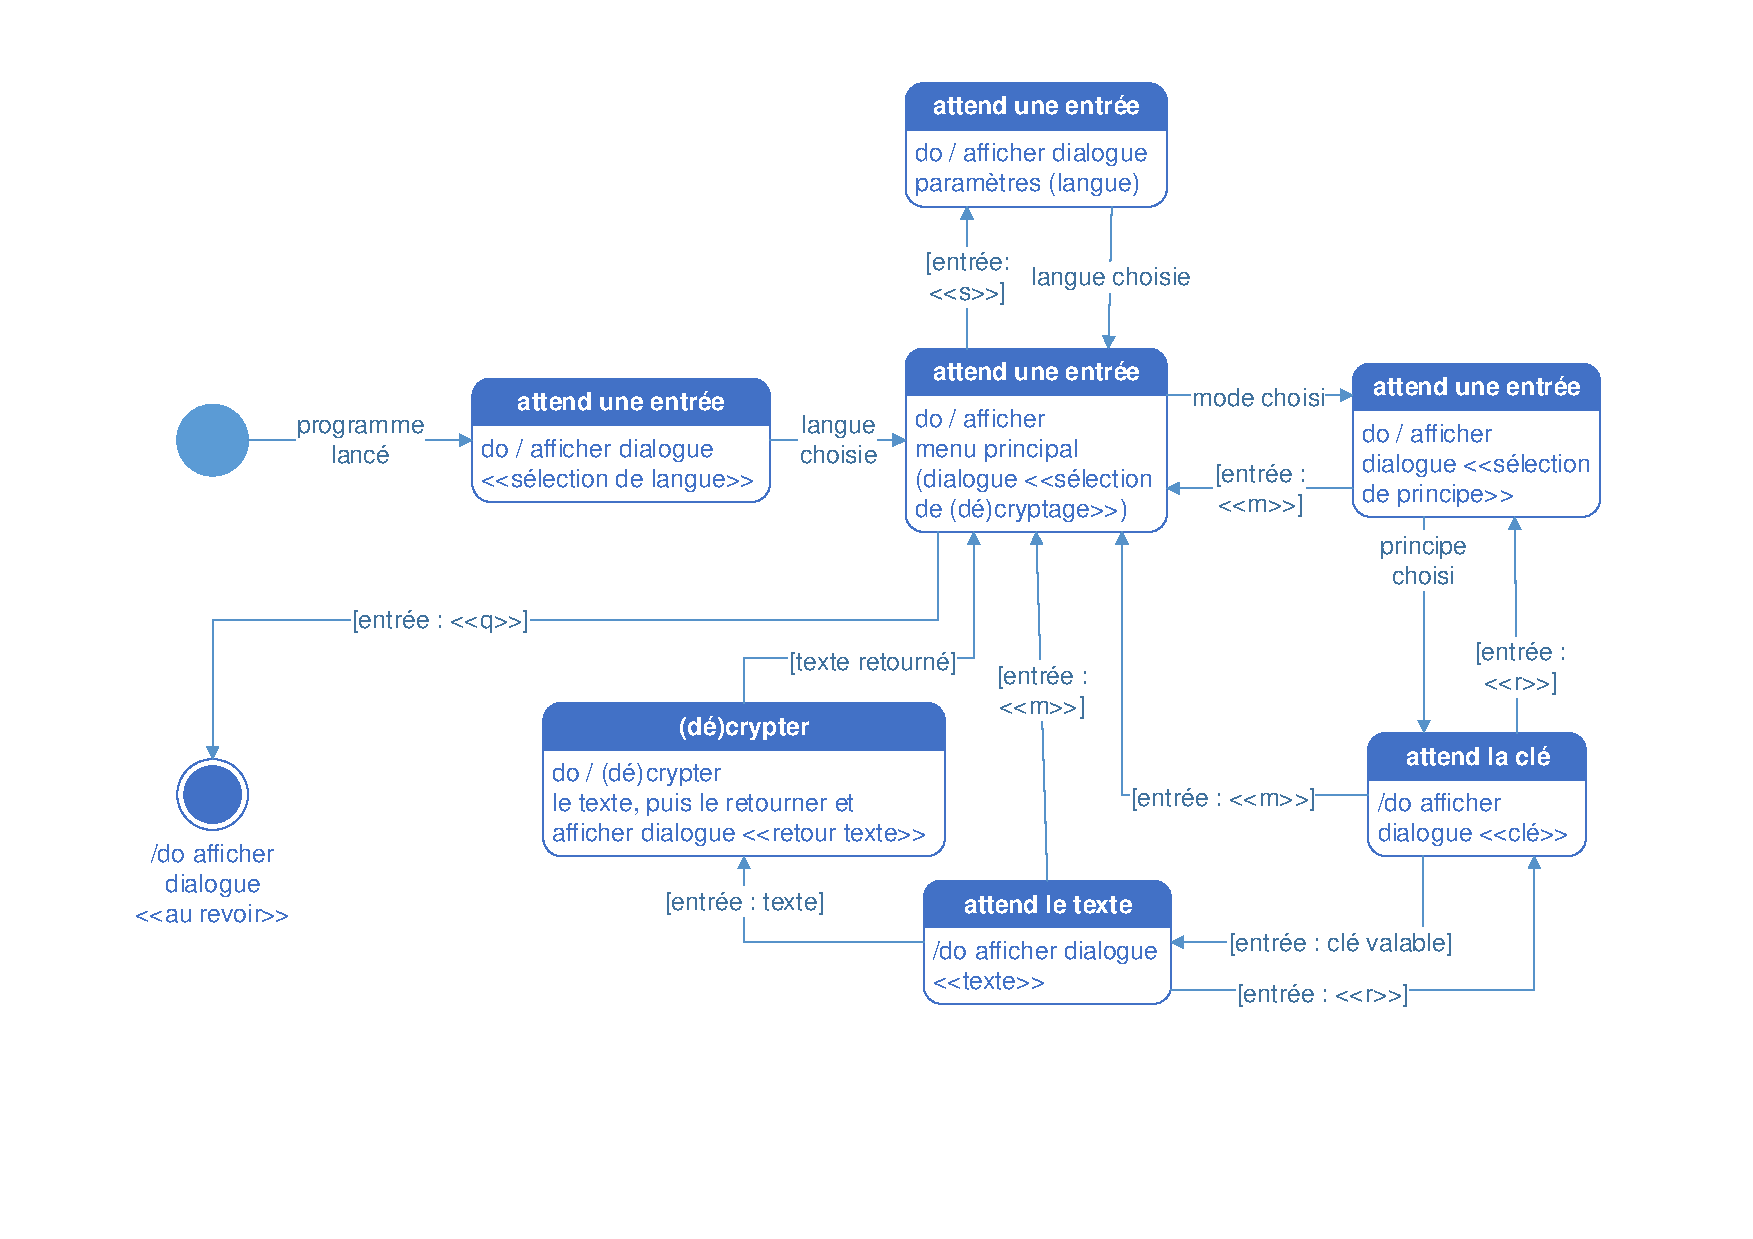
\includegraphics[width=\textwidth, trim=20mm 38mm 25mm 13mm, clip]{./Diagrammes/diagrammeDesEtats.pdf}
  %TRIM = LINKS UNTEN RECHTS OBEN
  %\caption{Différents états du programme}
	\label{img:etats}
\end{figure}

\subsection{En général}
\begin{itemize}
\item Quand l’utilisateur lance le programme on lui demande de choisir la langue, soit français, soit anglais.
\item Notre programme va proposer à l’utilisateur trois façons différentes de (dé)crypter un texte de complexité croissante et demander une clé.
\item Les différentes manières sont le principe du chiffre de César, du chiffre de Vigenère et de la machine Enigma.
\end{itemize}

\newpage
\subsection{En détail et coupé en modules}
\begin{itemize}
\item \textit{Avant de commencer le (de)cryptage :}\\
On va créer une méthode qui formatera le texte (enlever les accents, les caractères spéciaux, les signes de ponctuation et les espaces, puis mettre tout en majuscule).\\
\item \textit{(Dé)Cryptage César :}\\
On compte transformer les lettres du texte en nombres par le système unicode, ensuite on additionne la clé (nombre) aux nombres obtenus par le système.On reconvertit alors les lettres en caractères et retourne le texte.
Pour le décryptage, il suffit de soustraire au lieu d'additionner.\\
\item \textit{(Dé)Cryptage Vigenère :}\\
Dans un premier temps on crée une matrice de 26 x 26 lettres contenant l’alphabet représentant le tableau de Vigenère et une matrice à deux lignes pour le texte et la clé. Dans un deuxième temps on prend le texte et on insère tour à tour les caractères individuels dans la première ligne de la matrice et la clé dans la deuxième. Chaque lettre du texte doit être attribuée à un caractère de la clé (mot) ce qui est permis en répétant le mot tant qu’ils restent des lettres du texte.
Le cryptage est fait caractère par un caractère. Pour trouver la lettre cryptée on regarde en premier la lettre du texte et on cherche la colonne de la matrice qui appartient à la lettre et on la mémorise. Par la suite on considère le caractère de la clé auquel la lettre du texte est attribuée et on cherche la ligne de la matrice qui appartient au caractère. Dès qu’on a trouvé les deux, la lettre de la matrice qui est enregistré sur cette case est la lettre cryptée laquelle est mémorisée dans une chaîne de caractère. Lorsqu’on a crypté toutes les lettres du texte, on retourne la chaîne de caractère qui est le texte crypté.
Pour le décryptage, on possède la matrice à deux lignes avec le texte crypté sur une ligne et la clé répétée sur l’autre. Pour chaque lettre du texte crypté, on parcourt dans le tableau de Vigenère (matrice) la ligne correspondant à la lettre de la clé répétée et lorsqu’on  trouve la lettre cryptée cherchée on remonte la ligne pour obtenir le caractère décrypté correspondant à cette lettre. De la même manière que pour le cryptage on mémorise les lettres obtenues dans une chaîne de caractère ce qui permet d’avoir au final le message décrypté.\\
\item \textit{(Dé)Cryptage Enigma :}\\
Pour commencer nous créons cinq listes : La première correspond au tableau de permutation, les trois suivantes aux rotors au milieu et la dernière au réflecteur. Au début de la programmation on choisit un décalage fixe ; si possible on essayera plus tard de changer le décalage automatiquement.
Pour les connecteurs, il y en aura dix ainsi 20 lettres seront connectées entre elles et six qui ne le seront pas. Nous allons créer une fonction qui, si la lettre est connectée, va retourner la lettre associée.
On appelle ensuite des fonctions qui exécutent les décalages au niveau des trois rotors et après on utilise la fonction correspondant au réflecteur pour permuter les lettres. On repasse finalement à nouveau par les rotors et on obtient une certaine lettre. Si la lettre est connectée à une autre, on retourne l’autre lettre, sinon on garde la même, celle-ci est alors la lettre (dé)cryptée.\\
\end{itemize}

\newpage
\section{Interfaces utilisateurs}

{\fbox{\raggedright    %1
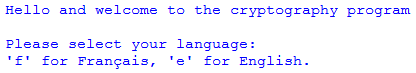
\includegraphics{./Pictures/interface/01_startScreen.png}}
	\captionof{figure}{Écran d'accueil}
}

\subsection{En anglais :}

{\fbox{\raggedright
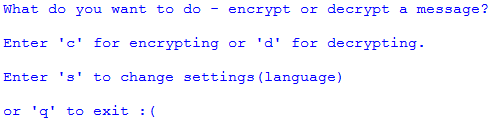
\includegraphics{./Pictures/interface/english/02_english_mainMenu.png}}	%2
\captionof{figure}{Menu principal}
%\medskip
\vspace{1cm}
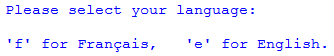
\includegraphics{./Pictures/interface/settingsDialogue.png}		%3
\captionof{figure}{Paramètres}
\vspace{1cm}
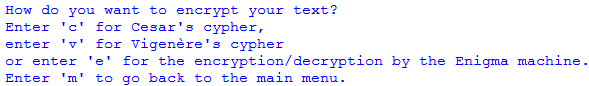
\includegraphics{./Pictures/interface/english/03_english_cryptage.png}	%4
\captionof{figure}{Cryptage}
\vspace{1cm}
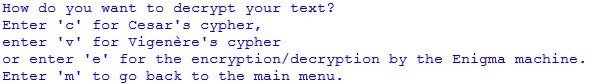
\includegraphics{./Pictures/interface/english/03_english_decryptage.png}	%5
\captionof{figure}{Décryptage}
\vspace{1cm}
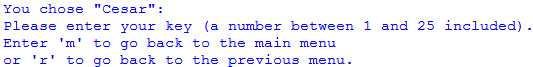
\includegraphics{./Pictures/interface/english/04_english_cesar.png}		%6
\captionof{figure}{Le chiffre de César}
\vspace{1cm}
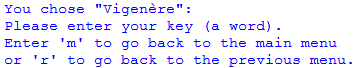
\includegraphics{./Pictures/interface/english/04_english_vigenere.png}	%7
\captionof{figure}{Le chiffre de Vigenère}
\vspace{1cm}
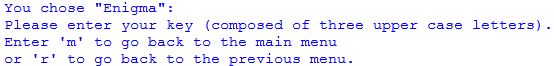
\includegraphics{./Pictures/interface/english/04_english_enigma.png}		%8
\captionof{figure}{Le cryptage par la machine Enigma}
\vspace{1cm}
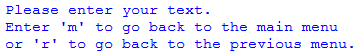
\includegraphics{./Pictures/interface/english/05_english_insertText.png}		%9
\captionof{figure}{Entrée du texte}
\vspace{1cm}
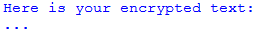
\includegraphics{./Pictures/interface/english/06_english_cryptage_showText.png}		%10
\captionof{figure}{Affichage du texte crypté}
\vspace{1cm}
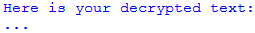
\includegraphics{./Pictures/interface/english/06_english_decryptage_showText.png}		%11
\captionof{figure}{Affichage du texte décrypté}
\vspace{1cm}
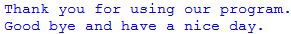
\includegraphics{./Pictures/interface/english/07_english_quitMessage.png}		%12
\captionof{figure}{Sortie du programme}
\vspace{1cm}
}
\newpage
\subsection{En français :}
{\raggedright
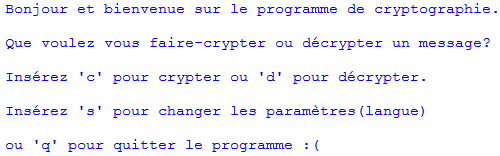
\includegraphics{./Pictures/interface/french/02_french_mainMenu.png}	%2
\captionof{figure}{Menu principal}
%\medskip
\vspace{1cm}
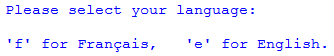
\includegraphics{./Pictures/interface/settingsDialogue.png}		%3
\captionof{figure}{Paramètres}
\vspace{1cm}
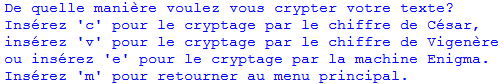
\includegraphics{./Pictures/interface/french/03_french_cryptage.png}	%4
\captionof{figure}{Cryptage}
\vspace{1cm}
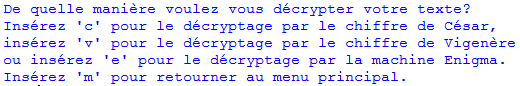
\includegraphics{./Pictures/interface/french/03_french_decryptage.png}	%5
\captionof{figure}{Décryptage}
\vspace{1cm}
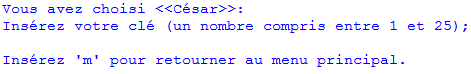
\includegraphics{./Pictures/interface/french/04_french_cesar.png}		%6
\captionof{figure}{Le chiffre de César}
\vspace{1cm}
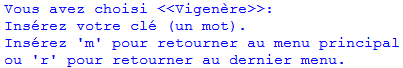
\includegraphics{./Pictures/interface/french/04_french_vigenere.png}	%7
\captionof{figure}{Le chiffre de Vigenère}
\vspace{1cm}
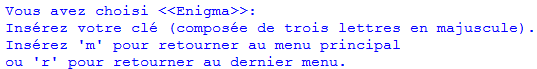
\includegraphics{./Pictures/interface/french/04_french_enigma.png}		%8
\captionof{figure}{Le cryptage par la machine Enigma}
\vspace{1cm}
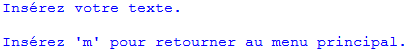
\includegraphics{./Pictures/interface/french/05_french_insertText.png}	%9
\captionof{figure}{Entrée du texte}
\vspace{1cm}
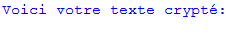
\includegraphics{./Pictures/interface/french/06_french_cryptage_showText.png}		%10
\captionof{figure}{Affichage du texte crypté}
\vspace{1cm}
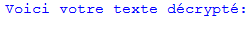
\includegraphics{./Pictures/interface/french/06_french_decryptage_showText.png}		%11
\captionof{figure}{Affichage du texte décrypté}
\vspace{1cm}
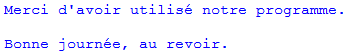
\includegraphics{./Pictures/interface/french/07_french_quitMessage.png}		%12
\captionof{figure}{Sortie du programme}
}







%(meist im CIE"=Normvalenzsystem)

%\begin{floatingfigure}[l]{5.3cm}
%	\includegraphics[width=0.25\textwidth]{./Bilder/2venn.png}
%	\caption{Prinzip der additiven Farbmischung}
%	\label{venn}
%\end{floatingfigure}


%\par
%\vspace{2em}
%\vspace{1em}

% "`Standard Definition Television"', HDTV für "`High Definition Television'".



%\begin{tabular}[t]{lr}
%Naher Osten & 65\%\\
%Lateinamerika & 13\%\\
%\end{tabular}\\

%\begin{itemize}
%\item \blindtext
%\item \blindtext
%\end{itemize}
%\begin{enumerate}
%\item \blindtext
%\item \blindtext
%\end{enumerate}
%\begin{description}
%\item [Ant] \blindtext
%\item [Elephant] \blindtext

%\textbf{greatest} 
%\underline{science} 
%\textbf{\textit{accident}}.


\end{document}




% LABEL UNTER CAPTION

